
\providecommand{\myrootdir}{..}
\documentclass[\myrootdir/main.tex]{subfiles}

\begin{document}

\chapter{Information Retrieval Techniques for Build Logs}
\plan{whole chapter: some reordering and reviewing to do, write about 3 pages about ir technique model classes and ir tasks and other techniques}
\plan{write, 1/3 page, blocked by: rest of chapter}
\label{sec:models}
%\includegraphics[page=1, width=\textwidth, trim={0.5cm 0.5cm 0.5cm 0.5cm}, clip]{img/RetreatSeptemberSlides.pdf}
Many different information retrieval techniques ... this section describes the conceptional / theoretical results of our thesis ...
We create a model to characterize BLIE techniques so we can discuss their similarities and differences more clearly.
Additionally we present a complimentary model for IE tasks, to describe use cases for BLIE techniques in a structured way.
From our analysis of build logs we share our notion of the retrievable information within a build log.

\begin{figure}[h]
	\centering
	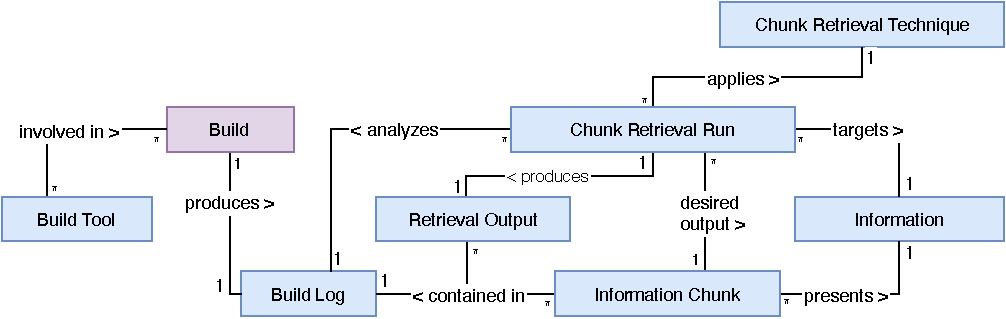
\includegraphics[width=\textwidth, clip]{img/build-overview.pdf}
	\caption{The different entities involved in a build}
	\label{fig:build-overview}
\end{figure}

\section{Characteristics of a Build Log}
\plan{citations needed, make clean figure of contribution of tools to log, 1 caro-review before finalized}
The idea of CI is, to integrate new software changes fast and often to catch errors early~\cite{humble2010continuous}.
After making a change, the developer commits and pushes it to a shared source code repository.
Companies often use a specific CI server, e.g.\ Travis CI, linked to their source code repository.
A CI build might then be triggered by a push on specific branches or after a pull request was created.
When such a CI build is triggered, it typically runs through these stages:

\begin{itemize}
	\item Pulling the new, changed version of the source code onto the server.
	\item Running static analysis tools~\cite{zampetti2017open}.
	\item Building the software, i.e. compiling and packaging it~\cite{phillips2014understanding}.
	\item Running automated tests~\cite{beller2017oops}.
	\item Deployment of the build artifact~\cite{schermann2016empirical}.
\end{itemize}

However these are only \emph{typical} stages and there is a high variability in the CI build processes of different software projects~\cite{staahl2014modeling}.
Some smaller projects might use CI to just make sure their code compiles as a minimal check before reviewing a pull request.
Other projects might have various stages of extensive automated testing.

Software tools involved in the build write out log messages to the console.
They communicate progress updates, error and warning messages to the user~\cite{yuan2012characterizing}.
We refer to to the sum of this output as build log.
The structure of their output is chosen by every tool themselves.
Many have implicit or explicit structuring rules, some adhere to predefined standards like RSpec or PHPUnit~\cite{phpunit2019logging,rspec2019format}.
Figure \ref{fig:tool-log-contribution} shows how different tools contribute to the whole build log.

\begin{figure}[h]
	\centering
	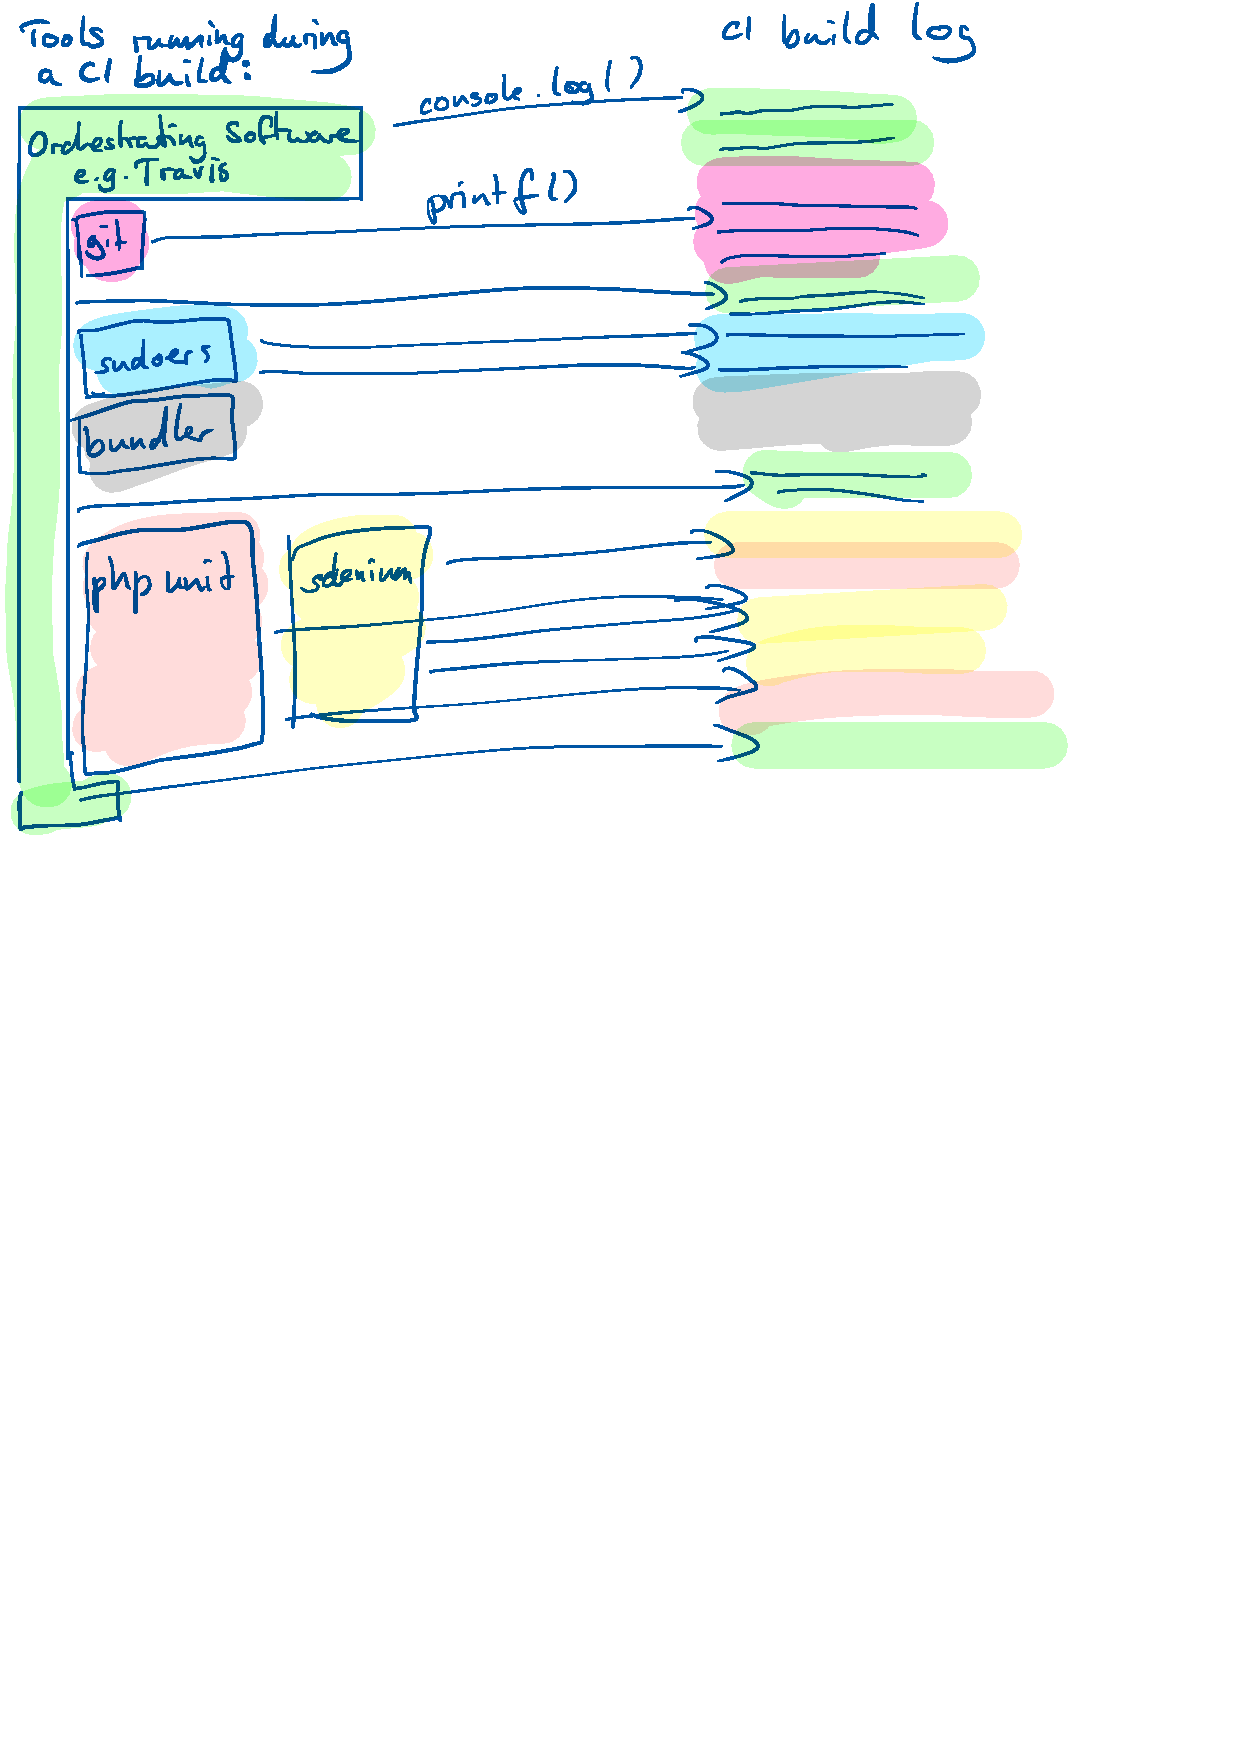
\includegraphics[width=\textwidth, trim={0cm 15cm 0cm 0cm}, clip]{img/tool-log-contribution.pdf}
	\caption{Contribution of different tools to the build log}
	\label{fig:tool-log-contribution}
\end{figure}

When analyzing build logs we might not have access to the exact build configuration, describing which tools are used in which order, or might not have access to a useable definition of the output structure of a specific tool.
As the structure of a build log is not known to us, we describe build logs as semi-structured. Section \ref{sec:rw-semi-structured-data} describes different properties of semi-structured data.


\section{Retrievable Information in Build Logs}
\plan{fix naming, then review again}
\begin{figure}[h]
	\centering
	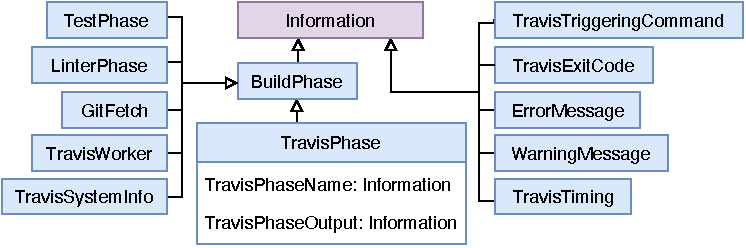
\includegraphics[width=\textwidth, clip]{img/build-log-information.pdf}
	\caption{Information retrievable from build logs}
	\label{fig:build-log-information}
\end{figure}
Continuous integration build logs contain a huge amount of information about the stages in the CI build they correspond to.
In this section we present a model, which more precisely describes our notion of a information retrievable from a CI build log.
Figure \ref{fig:build-log-information} shows the model.

The central class of our model is the \emph{BuildLogInformation} (BLI), representing an piece of information possibly retrievable from a build log.
\emph{Possibly}, because a BuildLogInformation is not necessarily present in every build log.
If it is present, we call it a \emph{BuildLogInformation instantiation} (BLII), which always relates to a specific build log, the one it is appearing in.

Each BLII for us has a \emph{textual representation} within the build log.
This textual representation is always a substring of the log text.
BuildLogInformations can be hierarchically ordered by their textual representations containing each other.
As this is an ad-hoc and a-posteriori structuring schema, as we describe in Section \ref{sec:rw-semi-structured-data}, the model only presents hierarchical ordering or containment for BuildLogInformations whose structure we definetely know.
Most build log information types can appear in various hierarchical arrangements and therefore not contained in any other type in the model.

During our initial exploration and log data collection for the \emph{Failing Build Log Data Set}, we collected a broad set of build logs from 29 languages and 87 repositories from Travis CI~\cite{travisci2019webpage}.
We inspected them to get an impression about the information one would want to retrieve from a build log.
Within the build logs from Travis CI we found different information types possibly interesting to be retrieved:

\begin{itemize}
	\item \textbf{BuildPhase} Build logs can be divided in the sections produced by different tools.
	      These build steps could be for example be a \texttt{TestPhase}, \textbf{LinterPhase}, \textbf{TravisWorker}, \textbf{GitFetch}, or \textbf{Sudoers} are some that we encountered in the logs.

	\item \textbf{TravisPhase} Travis CI build logs consists of several build phases defined within the Travis CI configuration language. Within the build log each of these steps are framed by \lstinline{travis_fold:start:<travis phase name>} and \\ \lstinline{travis_fold:end:<build step name>}.

	      A TravisPhase always contains:
	      \begin{itemize}
		      \item \textbf{TravisPhaseName} The string Travis CI uses to identify the phase within start and end statements.
		      \item \textbf{TravisPhaseOutput} The output generated during the build step. The textual representation of the \texttt{Build Step Output} Instantiation is the substring between the start and end statements.
	      \end{itemize}
	      You can see an example of a TravisPhase and its components within a build log in Figure \ref{fig:log-1}.

	\item
	\item \textbf{TravisTiming} Travis can measure the time of specified sections of the build process.
	      Timing information can be useful to retrieve when you want to automatically monitor the performance of your bui
	      You can see an example of a Travis Build Step and its components within a build log in Figure \ref{fig:log-1}.
	      %It represents those by \lstinline{travis_time:start:<timing section id>} and \\ \lstinline{travis_time:end:<timing section id>:start=<start time>,finish=<finish time>,duration=<duration>}

	\item \textbf{TravisWorker} Travis CI mentions for each build which machine is executing it.
	      Retrieving this information from multiple build logs could for example help visualize the impact of the build server assignment algorithm.
	      The TravisWorker is a good example to show that the same BLI can have different textual representations in different build logs.
	      You can see examples of TravisWorker instantiations in Figure \ref{fig:log-0} and Figure \ref{fig:log-2}.

	\item \textbf{TravisSystemInfo} At the beginning of each log Travis CI describes the tech stack of the server executing the build.
	      The system info could be retrieved from both failing and successful logs and compared to identify if a failure is possibly based on the execution environment.
	      You can see an example of a TravisSystemInfo instantiation within a build log in Figure \ref{fig:log-0}.

	\item \textbf{TriggeringCommand} Travis CI logs the commands it uses to call certain tools.
	      These come from the \texttt{travis.yml} configuring the build.
	      Retrieving this information from the log could for example be useful when reverse engineering the build configuration.
	      You can see an example of a TriggeringCommand instantiation within a build log in Figure \ref{fig:log-3}.

	\item \textbf{ExitCode} Travis CI prints all exit codes of commands.
	      This information could be used to fill an overview of the build steps and why they failed.
	      You can see an example of an ExitCode instantiation within a build log in Figure \ref{fig:log-3}.

	\item \textbf{ErrorMessage} Various tools involved in the build process might output messages of errors that occurred during their execution.
	      Retrieving these and showing them to developers could help them understand quicker why the build failed.
	      You can see an example of and ErrorMessage instantiation within a build log in Figure \ref{fig:log-3}.

	\item \textbf{WarningMessage} In addition to errors, tools also print warning messages.
	      These could be collected, counted and presented to developers, encouraging them to resolve them to improve their software.
	      You can see examples of WarningMessage instantiations within build logs in Figure \ref{fig:log-4} and Figure \ref{fig:log-5}.

\end{itemize}

\begin{figure}[hp]
	\centering
	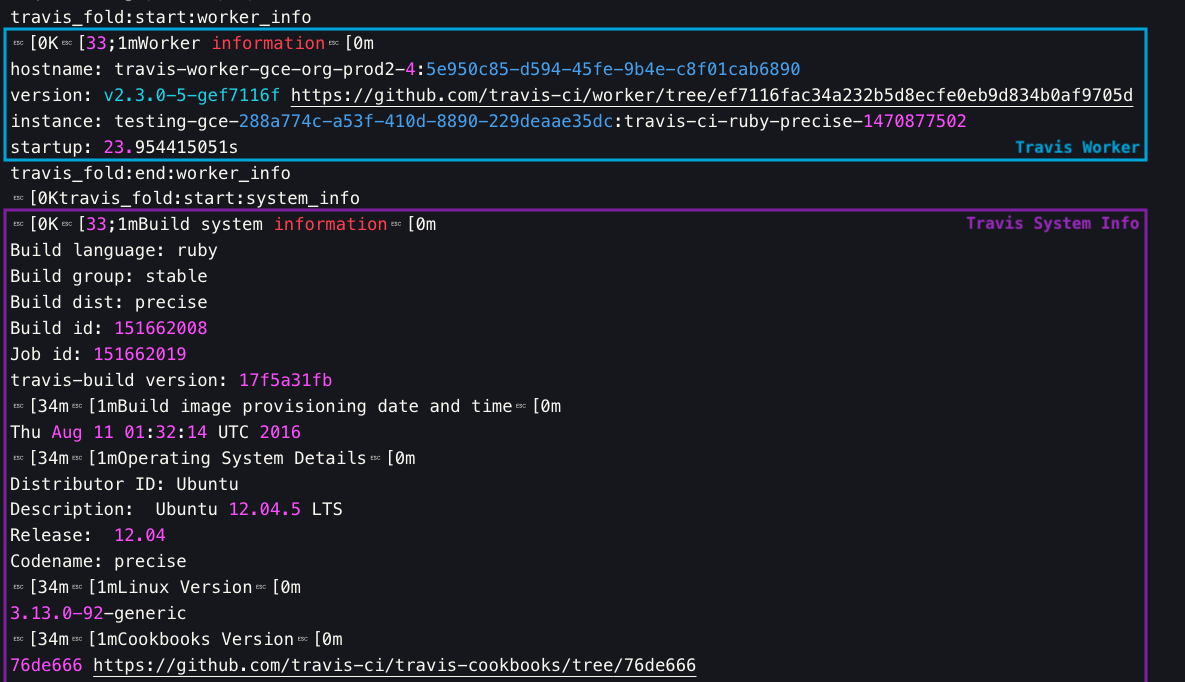
\includegraphics[width=\textwidth, clip]{img/log0.png}
	\caption{Excerpt from a build log showing textual representations of a long Travis Worker instantiation and a Travis System Info instantiation}
	\label{fig:log-0}
\end{figure}
\begin{figure}[hp]
	\centering
	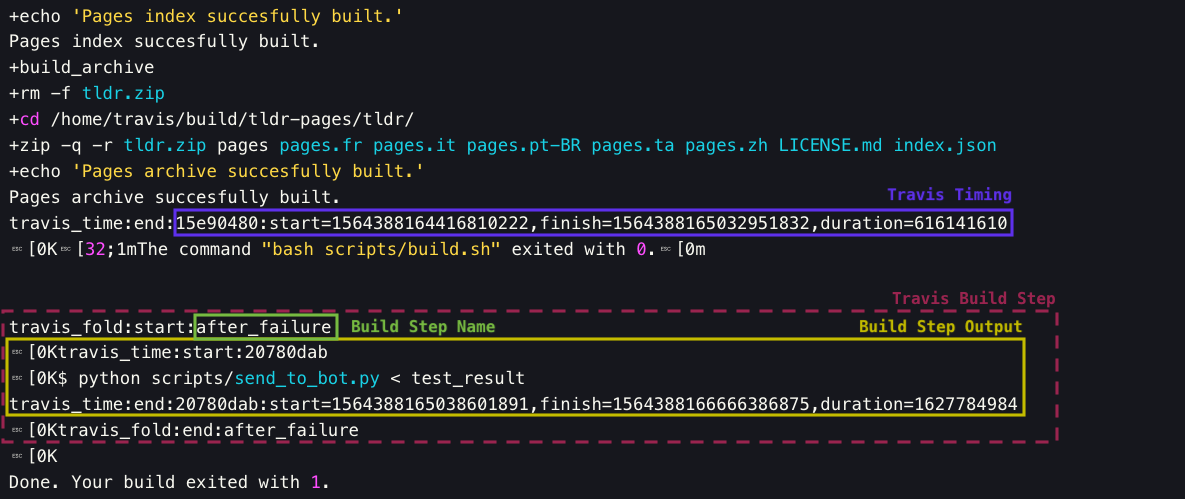
\includegraphics[width=\textwidth, clip]{img/log1.png}
	\caption{Excerpt from a build log showing textual representations of a Travis Timing instantiation and a Travis Build Step, containing the Build Step Name and the Build Step Output}
	\label{fig:log-1}
\end{figure}
\begin{figure}[hp]
	\centering
	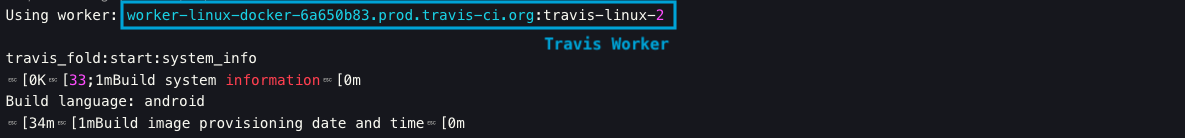
\includegraphics[width=\textwidth, clip]{img/log2.png}
	\caption{Excerpt from a build log showing textual representations of a short Travis Worker instantiation}
	\label{fig:log-2}
\end{figure}
\begin{figure}[hp]
	\centering
	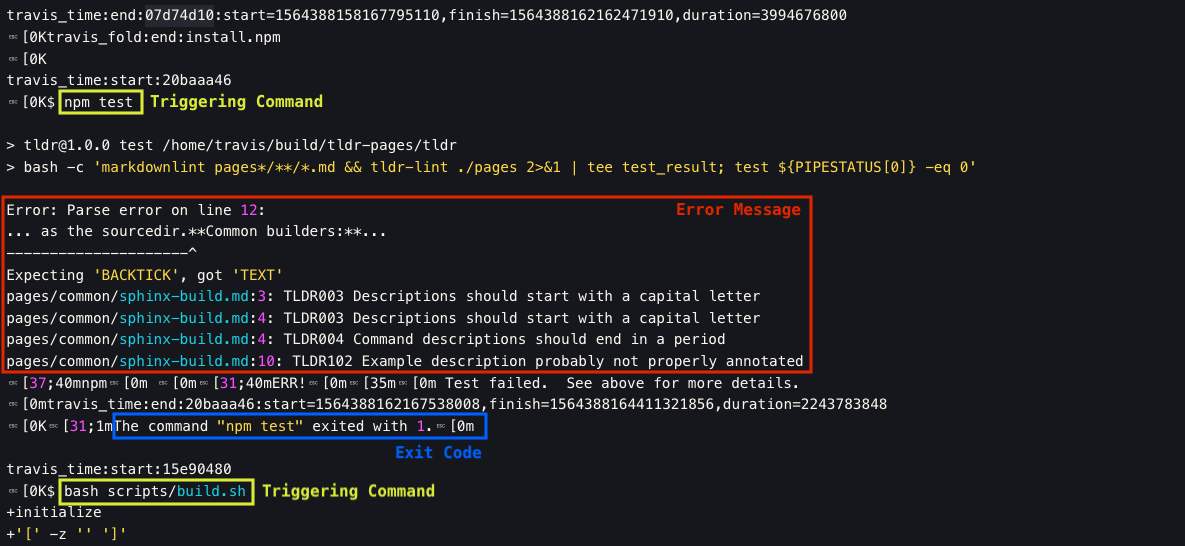
\includegraphics[width=\textwidth, clip]{img/log3.png}
	\caption{Excerpt from a build log showing textual representations of Error Message, Exit Code and Triggering Command instantiations}
	\label{fig:log-3}
\end{figure}
\begin{figure}[hp]
	\centering
	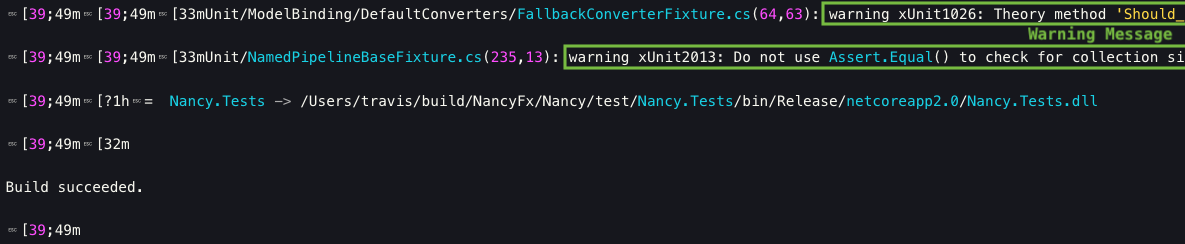
\includegraphics[width=\textwidth, clip]{img/log4.png}
	\caption{Excerpt from a build log showing textual representations of Warning Message instantiations}
	\label{fig:log-4}
\end{figure}
\begin{figure}[hp]
	\centering
	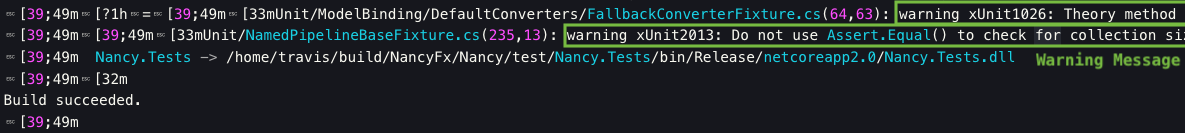
\includegraphics[width=\textwidth, clip]{img/log5.png}
	\caption{Excerpt from a build log showing textual representations of Warning Message instantiations}
	\label{fig:log-5}
\end{figure}


\section{Characteristics of Information Retrieval Techniques}
\plan{describe model classes, 1 page text}
\begin{figure}[h]
	\centering
	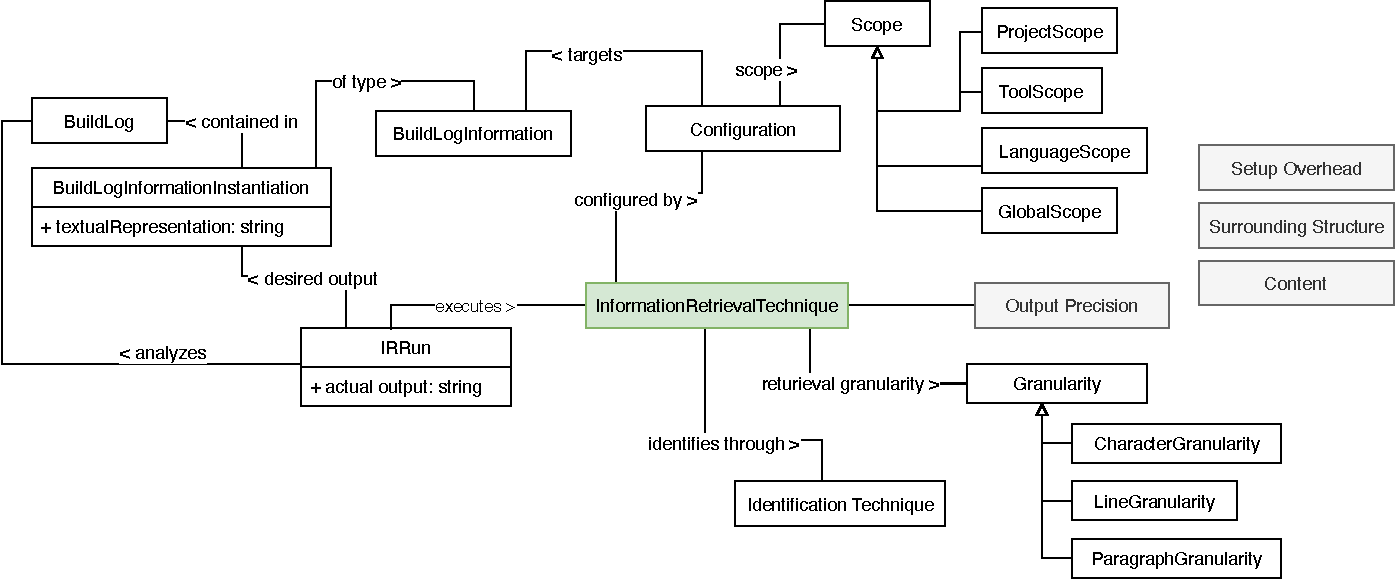
\includegraphics[width=\textwidth, clip]{img/ir-technique.pdf}
	\caption{Model for an Information Retrieval Technique}
	\label{fig:model-ie-technique}
\end{figure}
For this thesis we want to evaluate different information retrieval techniques when applied to CI build logs.
We focus on techniques that do not require to parse the structure of a whole build log, but rather focus on extracting just one specified information.
We refer to such a technique as BuildLogInformationRetrievalTechnique (BLIRT).

A BLIRT run consumes a build log (text file) and produces a certain output (text).

A BLIRT
\begin{itemize}
	\item targets a specific \textbf{BuildLogInformation}.
	\item identifies the text part to retrieve through an \textbf{IdentificationTechnique}.
	\item is configured by a \textbf{Configuration}
	      \begin{itemize}
		      \item each configuration addresses a specific \textbf{Scope}.
		            The Scope can be a specific project, a tool involved in the build, a programming language or global, configuring a retrieval technique for all possible build logs.
	      \end{itemize}
	\item can retrieve text passages with a specific \textbf{Granularity}, i.e. the smallest extractable text piece.
	      The Granularity can be at the level of characters, lines or paragraphs.
\end{itemize}

The last sections of this chapter show instantiations of this model for the three techniques we analyze and an additional one from related works.

\section{Information Retrieval Tasks}
\plan{what do we need here?, come up with model if we keep this, 1 page text max.}
Previous sections gave various examples of situations where a developer or a researcher wants to retrieve information from a build log.
The goal of this work is to clarify which BLIRT is suited for their specific task.
In this section we structure we present different important characteristics of such an IR task.
You can see the model in Figure \ref{fig:model-ir-task}

\begin{figure}[h]
	\centering
	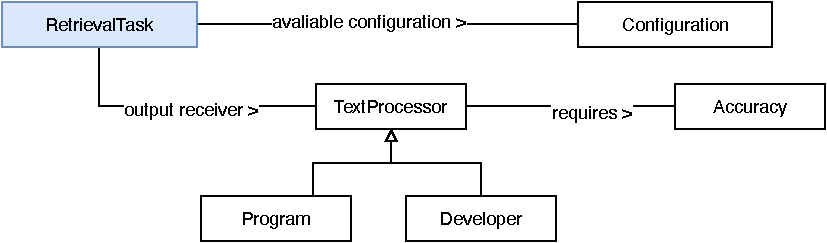
\includegraphics[width=\textwidth, clip]{img/ir-task.pdf}
	\caption{Model for an Information Retrieval Task}
	\label{fig:model-ir-task}
\end{figure}

A InformationRetrievalTask
\begin{itemize}
	\item has a specific amount and kind of \textbf{Configuration} available.
	      This represents how much data is available for the technique to learn what to extract.
	      For a BLIRT to be suited the available configuration has to match to needed configuration of the technique.
	\item is connected to a \textbf{TextProcessor} retrieving the output.
	      This can be for example a developer reading the output or a program.
	      Different TextProcessors require different accuracies in the output, e.g. a program needs exact retrievals to process automatically, while a developer can cope easier with falsely extracted lines.
\end{itemize}
\todo{give 2-3 concrete example instantiations here}


\begin{figure}[hp]
	\centering
	\begin{minipage}{0.45\textwidth}
		\centering
		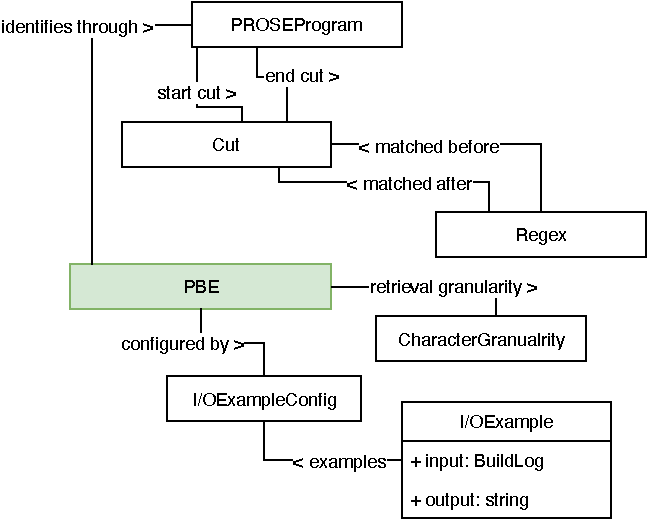
\includegraphics[width=\textwidth, clip]{img/pbe-technique.pdf}
		\caption{Synthesizing Regular Expression Programs by Example Using PROSE}
		\label{fig:prose-explanation}
	\end{minipage}\hfill
	\begin{minipage}{0.45\textwidth}
		\centering
		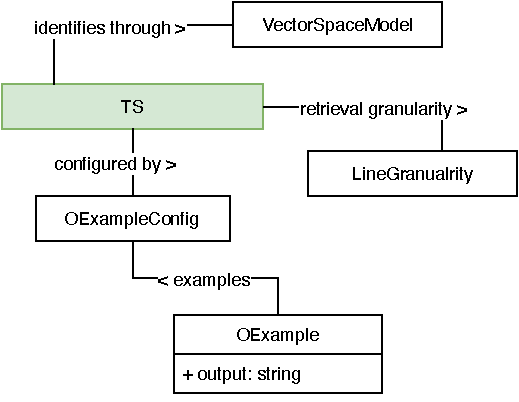
\includegraphics[width=\textwidth, clip]{img/ts-technique.pdf}
		\caption{Retrieving Information Using Text Similarity}
		\label{fig:text-similarity-explanation}
	\end{minipage}
\end{figure}

\section{PROSE Program Synthesis}
\plan{2 caro-reviews before finalized}

\subsection{Introduction}
\emph{Programming by Example (PBE)} is a technique where programs are synthesized according to in and output examples provided by the user.
It enables users to create programs without requiring programming knowledge~\cite{mayer2015user}.
Applied to the task of text extraction through regular expressions it relieves the developer from having to understand the whole document structure to solve a single extraction task~\cite{le2014flashextract:}.
We chose to investigate the applicability of generating regular expression programs by example to extracting information from build logs.
In this work we refer to our interpretation of this technique as \emph{PBE}.
In the following we will explain the concept of how we apply PBE to information retrieval from CI build logs, the concrete implementation is described in \ref{sec:impl-pbe}.
Figure \ref{fig:prose-explanation} shows the instantiation of the BLIRT model for PBE.

\subsection{Method}
In/Output examples (I/O examples) are the main driver of Programming by Example.
When extracting information from build logs the \emph{input} is always a whole build log, i.e. the whole text of the build log file without any preprocessing.
In the implementation we did have to apply a few text replacements as described in \ref{sec:impl-preprocessing}.
The \emph{output} is always a substring of the log file text, representing the substring that should be extracted by the synthesized program when given the corresponding input file.
One or multiple I/O examples are needed as configuration for PBE, they are used to define substring of a log should be extracted.Our approach is based on the Flash Extract DSL, which in turn is based on the FlashMeta algorithm. Both are described in Section \ref{sec:rw-prose}.
%For execution PBE takes a build file as input and returns a substring of the build file content.

\subsection{Perspective: Usability vs. Technical Aspects}
Generally, we are interested in whether a Programming by Example could replace manually writing regular expressions.
Writing and especially maintaining regular expressions is known to be a difficult, tedious and error-prone task~\cite{michael2019regexes}.
There are two ways to approach this question: from the usability side or the technical side.

When studying the applicability of PBE from the \emph{usability} perspective you run into questions like
\begin{itemize}
	\item Are users faster when using PBE compared to manual regex construction?
	\item Are users more comfortable using PBE over manual regex construction?
	\item Are users confident in the resulting regular expression program from PBE?
	\item Are the resulting extractions more or less accurate when using PBE over manual regex construction?
\end{itemize}
Some of these were already evaluated in existing works about PBE and user interaction~\cite{mayer2015user,lau2009why-programming-by-demonstration,miller2001outlier}.
Adequately answering those questions is however highly dependent on the user interface and the corresponding interaction model used during a study.
Developers who are accustomed to crunching on regular expressions in their favorite IDE or Editor might have an adversely negative view on synthesizing programs from examples in an unknow interface.
Mayer et al.~\cite{mayer2015user} presented two system-user interaction models to improve the confidence of users into the programs synthesized from their examples.
We feel such questions of usability can be answered separately from the application domain of build logs.

For our work we chose to look at the applicability of PBE from the \emph{technical} perspective.
We investigate whether current program synthesis techniques are able to learn programs for information retrieval tasks in the domain of CI build logs.
Furthermore we gather insights in how PBE has to be applied to yield useable results and perform best.
Our implementation of PBE, is mainly based on the Flash Extract DSL~\cite{le2014flashextract:} of the PROSE library by Microsoft~\cite{prose2019webpage}.
Due to that our technique of text extraction through regular expression programs synthesized is highly influenced by the capabilities of Flash Extract.

\section{Text Similarity}
\plan{2 caro-reviews before finalized}

\subsection{Overview}
Text Similarity approaches are more and more used to filter unstructured textual software artifacts~\cite{runeson2007detection,marcus2005recovery,antoniol2002recovering,mccarey2006recommending}.
One common and simple technique the Vector Space Model~\cite{schutze2008introduction}.
We investigate when it is a suitable technique to retrieve information from build logs.
In the following we will explain the concept of how we apply text similarity to information retrieval from CI build logs (TS), the concrete implementation is described in \ref{sec:impl-ts}.
Figure \ref{fig:text-similarity-explanation} shows the instantiation of the BLIRT model for TS.

\subsection{Method}
To configure a retrieval though text similarity we chose to use the same concept of I/O examples as for PBE.
The lines of the output strings of a given example set define our search query.

First, the search query is processed.
The output strings of the example set configuring the technique are split into single lines.
For each line we apply preprocessing: Splitting it into tokens, in our case words.
%Commonly text similarity techniques employ further normalization like removing special characters and stop words.
%We chose to keep the build log lines as complete as possible, as we often saw special characters and words identifying an interesting area.
Then we build a document-term-frequency matrix over the lines of the output strings and prune very often or very rarely appearing words.
Next, the algorithm applies term-frequency inverse document frequency, a best practice for natural language queries~\cite{lee1997document}.
To retrieve the desired information from a build log, we parse the whole text and process it in the same way.
The algorithm calculates the cosine simlarity~\cite{korenius2007principal} to compare each line of the build log with each line of the search query.
After summing up the similarities of each build log line to all the query lines, we sort the build log lines in decreasing similarity.
The average number of lines in the I/O example output strings determines how many of the most similar lines are returned as the output of the retrieval run.

%Information retrieval techniques are more and more prevalently used to extract textual information from unstructured textual sources~\mention{stuff annibale is referencing?}.

\begin{figure}[hp]
	\centering
	\begin{minipage}{0.45\textwidth}
		\centering
		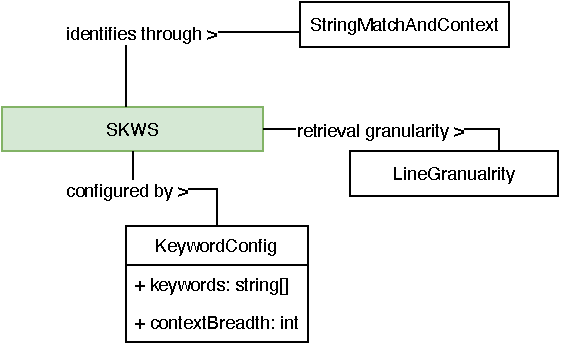
\includegraphics[width=\textwidth, clip]{img/skws-technique.pdf}
		\caption{Retrieving Information Using Simple Keyword Search}
		\label{fig:keyword-search-explanation}
	\end{minipage}\hfill
	\begin{minipage}{0.45\textwidth}
		\centering
		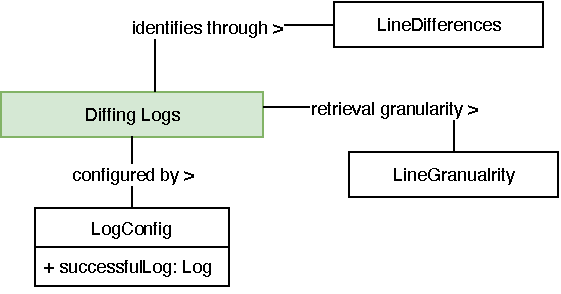
\includegraphics[width=\textwidth, clip]{img/diff-technique.pdf}
		\caption{Retrieving Information Using Amar et al.'s Line Diff Approach}
		\label{fig:diff-technique-model}
	\end{minipage}
\end{figure}

\section{Simple Keyword Search}
\plan{2 caro-reviews before finalized}

\subsection{Overview}
When we are looking for a specific information within a great amount of unstructured information, a first ad-hoc approach is to search for keywords in the text we assume to be near the information we are looking for.
This was one of the most common approaches we took when searching for the build failure reason within a log when creating our data set.
As this is a technique readily available in many tools developers use to view build logs, we want to study when such a simple search for keywords is recommendable for retrieving information from CI build logs.
In the following we will explain how we use simple keyword search to retrieve information from CI build logs (SKWS), the concrete implementation is described in \ref{sec:impl-skws}.
Figure \ref{fig:keyword-search-explanation} shows the instantiation of the BLIRT model for SKWS.

\subsection{Method}
SKWS is configured by giving a set of keywords.
For a retrieval run we then take a whole build log file as input and search for all exact occurrences of the keywords.
As keywords are often not directly describing the desired information but rather adjacent to the desired information, this technique not only retrieves the line with the keyword, but only the context around it.
We chose a context of 10 lines above and below the keyword appearance.

\section{Further Techniques}
\plan{decide: what to mention here, max 1 page text}

Amar et al. used a technique based on line diffs to retrieve relevant lines from a failed build log~\cite{amar2019mining}d \cite{amar2019mining}, as we describe in more detail in Section \ref{sec:rw-bl-analysis}
Figure \ref{fig:diff-technique-model} shows how this technique would be in our BLIRT model.


\end{document}
